\documentclass{beamer}
\mode<presentation>
{
  \usetheme{default}      % or try Darmstadt, Madrid, Warsaw, ...
  \usecolortheme{default} % or try albatross, beaver, crane, ...
  \usefonttheme{default}  % or try serif, structurebold, ...
  \setbeamertemplate{navigation symbols}{}
  \setbeamertemplate{caption}[numbered]
} 

\usepackage[english]{babel}
\usepackage[utf8]{inputenc}
\usepackage[T1]{fontenc}

\title[Your Short Title]{EE2227 Control Systems}
\author{Krati Arela}
\institute{EE18BTECH11050}
\date{\today}

\begin{document}

\begin{frame}
  \titlepage
\end{frame}

\section{Introduction}

\begin{frame}{Question 20/GATE EC-2015}


\begin{block}{Question}
A unity negative feedback system has the open loop transfer function\newline
\[G(s) = \frac{K}{s(s+1)(s+3)}\]\newline
The value of the gain K (>0) at which the root locus crosses the imaginary axis is ?
\end{block}

\end{frame}

\section{Solution}

\begin{frame}{Solution}
Given open loop transfer function\newline
\[G(s) = \frac{K}{s(s+1)(s+3)}\]\newline
we have P = 3 poles, at s = 0,-1,-3 and Z = 0 zeroes.
\newline
\newline
For unity negative feedback, closed loop transfer function is:\newline
\[T(s)= \frac{G(s)H(s)}{1+G(s)H(s)}\]\newline
Here H(s) = 1\newline
$\implies$\[T(s) = \frac{K}{s(s+1)(s+3)+K}\]

\end{frame}

\begin{frame}{Solution}
In the root locus diagram, we can observe the path of the closed loop poles\newline
Poles of closed loop transfer function are the roots of the Characteristic Equation.\newline
Characteristic Equation is:
\newline
\[ 1 + G(s)H(s) = 0\]\newline
$\implies$ \[ s^3 + 4s^2 + 3s + K = 0\] \newline
For the construction of root locus,
\textbf{If all elements of any row of the Routh array table are zero, then the root locus branch intersects the imaginary axis and vice-versa}\newline
\end{frame}

\begin{frame}{Solution}

\begin{table}
\centering
\begin{tabular}{l|r r}
Routh Array Table:
Order & Coefficients\\\hline
$s^3$ & 1 & 3 \\
$s^2$ & 4 & K \\
$s^1$ & (12-K)/4 & 0\\
$s^0$ & K & 
\end{tabular}

\end{table}

For poles to be on imaginary axis, row $s^1$ should be zero.\newline
So, \[\frac{12-K}{4} = 0\]
\newline Hence, $$\textbf{K = 12}$$


\end{frame}

\begin{frame}{Solution}
\begin{figure}
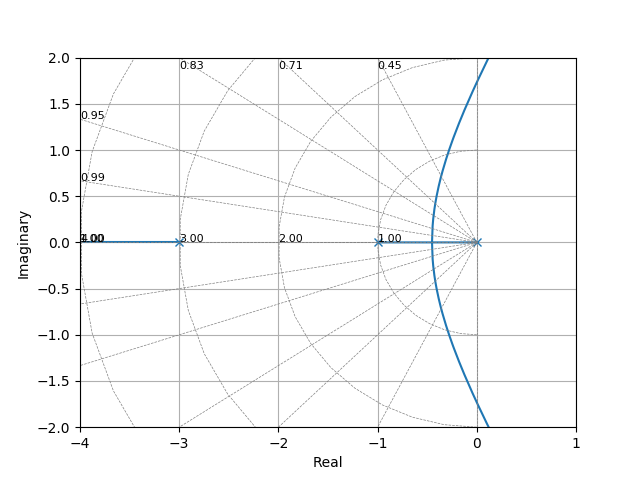
\includegraphics[width=250 pt]{Root_Locus.png}
\caption{\label{fig:your-figure}Root Locus Plot}
\end{figure}


\end{frame}

\end{document}
